% book example for classicthesis.sty
\documentclass[
  % Replace twoside with oneside if you are printing your thesis on a single side
  % of the paper, or for viewing on screen.
  oneside,
  %twoside,
  11pt, a4paper,
  footinclude=true,
  headinclude=true,
  cleardoublepage=empty
]{scrbook}

\usepackage{dissertation}
%---
\usepackage[T1]{fontenc}
\usepackage{textcomp}

\usepackage{listings}
\usepackage{xcolor}
\usepackage{pgfplots}
% \usepackage[miktex]{gnuplottex}
\usepackage{tikz}
% \usepackage{gnuplot-lua-tikz}
% \usepackage{mathpazo}
\pgfplotsset{width=10cm,compat=1.9}
% We will externalize the figures
\usepgfplotslibrary{external}
\tikzexternalize
%---
\usepackage[titles]{tocloft}
%% Aesthetic spacing redefines that look nicer to me than the defaults.
\setlength{\cftbeforechapskip}{2ex}
\setlength{\cftbeforesecskip}{0.5ex}
%% Use Helvetica-Narrow Bold for Chapter entries
\renewcommand{\cftpartfont}{%
  \fontsize{12}{14}\usefont{OT1}{phv}{bc}{n}\selectfont
}
\renewcommand{\cftchapfont}{%
  \fontsize{11}{13}\usefont{OT1}{phv}{bc}{n}\selectfont
}
\renewcommand{\cftsecfont}{%
  \fontsize{10}{11}\usefont{OT1}{phv}{}{n}\selectfont
}
\renewcommand{\cftsubsecfont}{%
  \fontsize{9}{10}\usefont{OT1}{phv}{}{n}\selectfont
}
\renewcommand{\cftfigfont}{%
  \fontsize{9}{10}\usefont{OT1}{phv}{}{n}\selectfont
}
\renewcommand{\cfttabfont}{%
  \fontsize{9}{10}\usefont{OT1}{phv}{}{n}\selectfont
}
%---

\definecolor{codegreen}{rgb}{0,0.6,0}
\definecolor{codegray}{rgb}{0.5,0.5,0.5}
\definecolor{codepurple}{rgb}{0.58,0,0.82}
\definecolor{backcolour}{rgb}{0.95,0.95,0.92}
\definecolor{s_orange}{HTML}{ef821c}
\definecolor{s_gray}{HTML}{8292A1}
\definecolor{s_line_gray}{HTML}{8e8f90}

\lstdefinestyle{mystyle}{
    backgroundcolor=\color{backcolour},   
    commentstyle=\color{codegreen},
    keywordstyle=\color{magenta},
    numberstyle=\tiny\color{codegray},
    stringstyle=\color{codepurple},
    basicstyle=\ttfamily\footnotesize,
    breakatwhitespace=false,         
    breaklines=true,                 
    captionpos=b,                    
    keepspaces=true,                 
    numbers=left,                    
    numbersep=5pt,                  
    showspaces=false,                
    showstringspaces=false,
    showtabs=false,                  
    tabsize=2
}
\lstset{style=mystyle}

\newcommand{\eqname}[1]{\tag*{#1}}% Tag equation with name

%usepackage[scaled=.92]{helvet}
\usepackage[all]{xy}
\usepackage{circuitikz}
% \usepackage[sorting=none,style=numeric]{biblatex}

% Title

\titleA{Study on FFT on the GPU}
% \titleB{Second line in title (if any)}
% \titleC{Third  line in title (if any)}

% Author

\author{Jorge Francisco Teixeira Bastos da Mota}

% Supervisor(es)

\supervisor{Supervisor}

\cosupervisor{Co-supervisor (if any)}

% Date

\date{\myear} % change to text if date is not today

\makeglossaries  %  either use this ...

\makeindex	% ... or this

\begin{document}\fontfamily{phv}\fontseries{mc}\selectfont
    
% Add acronym definitions
    
% Cover page ---------------------------------------------
%	\thispagestyle{empty}
    %!TEX root = dissertation.tex

\makeatletter

% UM_ENg Logo
\def\UMEng#1#2{\begin{tikzpicture}[
	% bars styling,
	logone/.style={rectangle,fill=white,rounded corners=0.08cm,minimum width=0.16cm,inner sep=0pt},
	bigone/.style={minimum height=0.74cm},
	smaone/.style={minimum height=0.48cm},
	engone/.style={minimum height=0.86cm},
	pos1/.style={xshift=1.3cm,yshift=1.3cm},
	pos2/.style={xshift=3.9cm,yshift=1.3cm}]
	
% Uminho logo
	\fill[fill=#1] (0,0) -- (2.6,0) -- (2.6,2.6) -- (0,2.6) -- cycle;
	\foreach \i in {1,...,3}{
		\node at (\i*120+30:0.45)[logone,bigone,pos1,rotate=\i*120-60]{};
		\node at (\i*120+90:0.60)[logone,smaone,pos1,rotate=\i*120]{};
	}

% EngUminho logo
	\fill[fill=#2] (2.6,0) -- (5.2,0) -- (5.2,2.6) -- (2.6,2.6) -- cycle;
	\foreach \i in {1,...,5}
		\node at (\i*72-90:0.74)[engone,logone,pos2,rotate=\i*72-90]{};
\end{tikzpicture}}

\def\yyy#1{\fontfamily{phv}\fontseries{mc}\selectfont {\ifnum\hide=1\relax\else#1\fi}}
\def\xxx#1{\fontfamily{phv}\fontseries{mc}\selectfont #1}
\def\zzz#1{\fontfamily{phv}\fontseries{mc}\fontseries{b}\selectfont #1}
\def\kkk#1{\fontfamily{phv}\fontseries{mc}\fontseries{b}\selectfont {\ifnum\hide=1\relax\else#1\fi}}

\long\def\coverEtc{
%Logo
~\vskip-4.1cm\rule{4cm}{0pt}\begin{tabular}{l}
\UMEng\umc{eng}
\\\zzz{Universidade do Minho}\rule{0pt}{1cm}
\\\xxx{}{Escola de Engenharia}
\\\xxx{Departamento de  Informática}
\\\rule{0pt}{4cm}
\\\xxx{{\Large\@author}}
\\\rule{0pt}{1em}
\\\zzz{\Large\@titleA}
\\\zzz{\Large\@titleB}
\\\zzz{\Large\@titleC}
\\\rule{0pt}{5cm}
\\\yyy{\large Master dissertation}
\\\yyy{\large Integrated Master’s in Informatics Engineering}
\\\rule{0pt}{6mm}
\\\yyy{\large Dissertation supervised by}
\\\kkk{\@supervisor}\rule{0pt}{4mm}
\\\kkk{\@cosupervisor}
\\\rule{0pt}{4.2cm}
\\\xxx{{\small\@date}}
\end{tabular}
}


\begin{frontcover}
\gdef\umc{um}\gdef\hide{1}
\thispagestyle{empty} \pagecolor{white} \textcolor{black} \coverEtc
\end{frontcover}

\begin{titlepage}
\gdef\umc{um}
\gdef\hide{0}
\thispagestyle{empty} \pagecolor{white}\textcolor{grey} \coverEtc
\end{titlepage}

\makeatother


%rm
    \cleardoublepage
%---------------------------------------------------------
    \pagenumbering{alph}
    \setcounter{page}{0}
%---------------------------------------------------------

%%%%%%%%%%%%%%%%%%%%%%%%%%%%%%%%%%%%%%%%%%%%%%%%%%%%%%%%%%%%%%%%%

% NOTES:
% There are some commented chapters and sections to improve readability when writing the dissertation
% In the end some of those chapters could or could not be included in the final pre-dissertation submission

%%%%%%%%%%%%%%%%%%%%%%%%%%%%%%%%%%%%%%%%%%%%%%%%%%%%%%%%%%%%%%%%%

% \chapter*{Copyright and Terms of Use for Third Party Work}

% This dissertation reports on academic work that can be used by third parties as long as the internationally accepted standards and good practices are respected concerning copyright and related rights.
% \vskip 1em
% \noindent This work can thereafter be used under the terms established in the license below.
% \vskip 1em
% \noindent Readers needing authorization conditions not provided for in the indicated licensing should contact the author through the RepositóriUM of the University of Minho.

%%%%%%%%%%%%%%%%%%%%%%%%%%%%%%%%%%%%%%%%%%%%%%%%%%%%%%%%%%%%%%%%%

% \section*{License granted to users of this work:}

% \CCBY % or replace by one in***************** the list below, cf https://alunos.uminho.pt/PT/estudantes/Formataes/3_Despacho_RT-31_2019_Anexo%203-Informa%c3%a7%c3%a3o-Direitor%20de%20Autor.docx 
%---------
%\CBYNCND
%\CCBYNCSA
%\CCBYNC
%\CCBYND
%\CCBYSA


%%%%%%%%%%%%%%%%%%%%%%%%%%%%%%%%%%%%%%%%%%%%%%%%%%%%%%%%%%%%%%%%%

% \chapter*{Acknowledgements}
% Write your acknowledgements here. Do not forget to mention the projects and grants that you have benefited from while doing your research, if any. Ask your supervisor about the specific textual format to use. (Funding agencies are quite strict about this.) 

% 	\cleardoublepage
    
%%%%%%%%%%%%%%%%%%%%%%%%%%%%%%%%%%%%%%%%%%%%%%%%%%%%%%%%%%%%%%%%%

% \chapter*{Statement of Integrity}

% I hereby declare having conducted this academic work with integrity.
% \vskip 1em\noindent
% I confirm that I have not used plagiarism or any form of undue use of information or falsification of results along the process leading to its elaboration. 
% \vskip 1em\noindent
% I further declare that I have fully acknowledged the Code of Ethical Conduct of the University of Minho.

%%%%%%%%%%%%%%%%%%%%%%%%%%%%%%%%%%%%%%%%%%%%%%%%%%%%%%%%%%%%%%%%%

\chapter*{Abstract}
    Write abstract here (en) or import corresponding file

\paragraph{Keywords} keywords, here, comma, separated.

    \cleardoublepage

%%%%%%%%%%%%%%%%%%%%%%%%%%%%%%%%%%%%%%%%%%%%%%%%%%%%%%%%%%%%%%%%%

\chapter*{Resumo}
    Escrever aqui resumo (pt) ou importar respectivo ficheiro
    
\paragraph{Palavras-chave} palavras, chave, aqui, separadas, por, v\'{\i}rgulas


    \cleardoublepage
    
    \pagenumbering{roman}
    \setcounter{page}{3}
    %pagestyle{fancy}   % -------- removed
    
    % Document
    \cleardoublepage
    \phantomsection
    % Adds 'Contents' to Contents chapter
    % \addcontentsline{toc}{chapter}{Contents}
    \tableofcontents
    
    % \cleardoublepage
    % \listoffigures
    
    % \cleardoublepage
    % \listoftables
    
    % \cleardoublepage
    % \lstlistoflistings
    
    % Add list of acronyms
    \cleardoublepage
    \pagenumbering{arabic}
    \setcounter{page}{5}

%%%%%%%%%%%%%%%%%%%%%%%%%%%%%%%%%%%%%%%%%%%%%%%%%%%%%%%%%%%%%%%%%

\chapter{Introduction}

\section{Contextualization}

%TODO: 
Empty

\section{Motivation}

%TODO: 
Empty

\section{Objectives}

The main objective of this dissertation is to provide efficient FFT alternatives in GLSL compared with dedicated tools for high performance of FFT computations like NVIDIA cuFFT library, while analysing the intrinsic of a good Fast Fourier Transform implementation on the GPU.
To accomplish the main objective there are two stages taken in consideration, "\textit{Analysis of CUDA and GLSL kernels}" to be well settled in their differences and to have a reference for the second stage "Analysis of cuFFT and GLSL FFT" which will cluster the study's main objective.

To compose a final verdict conclusion, we will use as case of study applications with implementation of the FFT in the field of Computer Graphics that require realtime performance.

\section{Document Organization}

%TODO: 
Empty
% A reaader with a good understanding of how the FFT works can skip to chapter <chaper_name>

%%%%%%%%%%%%%%%%%%%%%%%%%%%%%%%%%%%%%%%%%%%%%%%%%%%%%%%%%%%%%%%%%

\chapter{State of the Art}

\section{Fourier Transform}

\subsection{What is Fourier Transform}

The \textbf{Fourier Transform} is a mathematical method to transform the domain refered to as \textit{time} of a function, to the \textit{frequency} domain, intuitively the Inverse Fourier Transform is the corresponding method to reverse that process and reconstruct the original function from the one in \textit{frequency} domain representation.

Although there are many forms, the Fourier Transform key definition can be described as:

% Forward Fourier Transform
%FIXME: This equations are replacing the reference number for the name with '\eqname'
% It must show the name AND the number
\begin{equation} \label{eq1}
    % \begin{split}
    X(f) = \int_{-\infty}^{+\infty} x(t)e^{-i f t} dt \\ \eqname{Forward Fourier Transform} \\
    % \end{split}
\end{equation}

% Invense Fourier Transform
%FIXME: This equations are replacing the reference number for the name with '\eqname'
% It must show the name AND the number
\begin{equation} \label{eq2}
        x(t) = \frac{1}{2\pi} \int_{-\infty}^{+\infty} X(f)e^{-i f t} df \\ \eqname{Inverse Fourier Transform} \\
\end{equation}

% REVIEW
\begin{itemize}
    \item \( x(t), \forall t \in \mathbb{R} \rightarrow \) function in \textit{time} domain representation with real \( t \).
    \item \( X(f), \forall f \in \mathbb{R} \rightarrow \) function in \textit{frequency} domain representation with real \( f \), also called the Fourier Transform of \( x(t) \)
    \item \( i \rightarrow \) imaginary unit \( i = \sqrt{-1} \)
\end{itemize}

This formulation shows the usage of complex-valued domain since the imaginary unit \( i \) doesn't represent a value in the set of real numbers, making the fourier transform range from real to complex values, one complex coefficient per frequency \( X : \mathbb{R} \rightarrow \mathbb{C} \) 

If we take into account the Euler's formula, we can replace the Fourier Transform for an equivalent, fragmenting the euler constant for a sine and cosine

% Euler's Formula
\begin{equation} \label{euler_formula}
    e^{ix} = \cos x + i \sin x \\ \eqname{Euler's Formula} \\
\end{equation}

% Forward Fourier Transform with Euler's Formula
\begin{equation}
    X(f) = \int_{-\infty}^{+\infty} x(t) (\cos (-f t) + i \sin (-f t)) dt \\
\end{equation}

Hence, we can break the Fourier Transform apart into two formulas that give each coefficient of the sine and cosine components as functions without dealing with complex numbers.

% Forward Fourier Transform sine and consine
\begin{equation}
    \begin{split}
        X_{a}(f) = \int_{-\infty}^{+\infty} x(t) \cos (f t) dt \\
        X_{b}(f) = \int_{-\infty}^{+\infty} x(t) \sin (f t) dt \\
    \end{split}
\end{equation}


% FIXME: This might also be applied to the Inverse, study this later and try to deduce the correspondant pair of formulas
% NOTE: This is important for future reference

% Fourier's original formulation of the transform did not use complex numbers, but rather sines and cosines. % Chatfield, Chris (2004), The Analysis of Time Series: An Introduction, Texts in Statistical Science (6th ed.), London: Chapman & Hall/CRC, ISBN 9780203491683.

% TODO: explain the formula better
The above definition of the Fourier Integral \autoref{eq1} can only be valid if the integral exists for every value of the parameter \(f\). This model of the fourier transform applied to infinite domain functions is called \textbf{Continous Fourier Transform} and its targeted to the calculation of the this transform directly to functions with only finite discontinuities in \( x(t) \).

\subsection{Where it is used} \label{subsec:where_it_is_used}

It's noticieable the presence of Fourier Transforms in a great variety of apparent unrelated fields of application, even the FFT is often called ubiquitous\footnote{present, appearing, or found everywhere.} due to its effective nature of solving a great hand of problems for the most intended complexity time. Some of the fields of application include Applied Mechanics, Signal Processing, Sonics and Acoustics, Biomedical Engineering, Instrumentation, Radar, Numerical Methods, Electromagnetics, Computer Graphics and more \cite{brigham1988fast}.

One of the most well known cases of application is \textbf{Signal Analysis}, the Fourier Transform is probably the most important tool for analyzing signals, when representing a signal with amplitude as function of time, a signal can be translated to the frequency domain, a domain that consists of signals of sines and consines waves of varied frequencies, but to calculate the coefficients of those waves we need to use the Fourier Transform.

\begin{figure}[h]
    \centering
    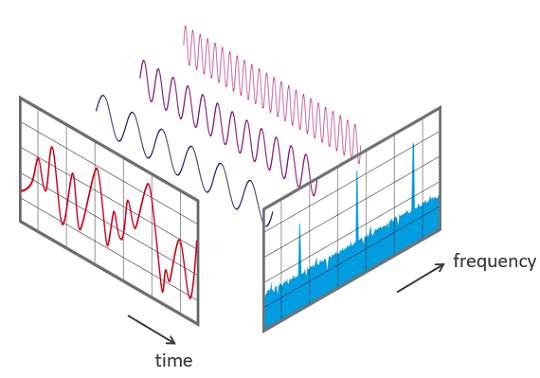
\includegraphics[width=0.5\textwidth]{imgs/fft_time_freq.png}
    \caption{Time to frequency signal decomposition}
\end{figure}

% REVIEW
Since the sines and consines waves are in simple waveforms they can then be manipulated with relative ease. This process is constantly present in communications since the transmission of data over wires and radio circuits through signals and most devices nowadays perform ir frequently


% TODO:
% - Elaborate more
% - Maybe describe the polynomial multiplication too
% - Move the 'jia2014polynomial' citation
% . . .

And much more applications such as polynomial multiplication \cite{jia2014polynomial}, numerical integration, time-domain interpolation, x-ray diffracition ...

% \begin{tikzpicture}
%   \begin{axis}[
%       axis lines = left,
%       xlabel = \(x\),
%       ylabel = {\(f(x)\)},
%   ]
%   %Below the red parabola is defined
%   \addplot [
%       domain=-10:10, 
%       samples=100, 
%       color=red,
%   ]
%   {x^2 - 2*x - 1};
%   \addlegendentry{\(x^2 - 2x - 1\)}
%   %Here the blue parabola is defined
%   \addplot [
%       domain=-10:10, 
%       samples=100, 
%       color=blue,
%       ]
%       {x^2 + 2*x + 1};
%   \addlegendentry{\(x^2 + 2x + 1\)}
  
%   \end{axis}
%   \end{tikzpicture}
% Dar 2 exemplos principais de como é aplicado e uma breve explicação
% - Signal processing

% Denote in the end that we'll use a different case of application for this comparisson (might not be true since we could use the image processing case as study)


\subsection{Discrete Fourier Transform}
% \section{Discrete Fourier Transform}

The Fourier Transform of a finite sequence of equally-spaced samples of a function is the called the \textbf{Discrete Fourier Transform} (DFT), it converts a finite set of values in \textit{time} domain to \textit{frequency} domain representation. Its the most important type of transform since it deals with a discrete amount of data and has the popular algorithm in which is the center of attention of fourier transforms, which can be implemented in machines and be computed by specialized hardware.

% Forward Discrete Fourier Transform
%FIXME: This equations are replacing the reference number for the name with '\eqname'
% It must show the name AND the number
\begin{equation} \label{eq3}
    X_{k} = \sum_{n=0}^{N-1}x_{n} \cdot e^{- \frac{i 2 \pi}{N}kn} \\ \eqname{Forward Discrete Fourier Transform} \\
\end{equation}

% Inverse Discrete Fourier Transform
%FIXME: This equations are replacing the reference number for the name with '\eqname'
% It must show the name AND the number
\begin{equation} \label{eq4}
    x_{n} = \frac{1}{N} \sum_{k=0}^{N-1}X_{k} \cdot e^{\frac{i 2 \pi}{N}kn} \\ \eqname{Inverse Discrete Fourier Transform} \\
\end{equation}

% REVIEW (english)
Notably, the discrete version of the Fourier Transform has some obvious differences since it deals with a discrete time sequence, the first difference is the sum covers all elements of the input values instead of integrating the infinite domain of the function, but we can also notice that the exponential, similar to the aforesaid, divides the values by \(N\) (\(N\) being the total number of elements in the sequence) due to the inability to look at frequency and time \(ft\) continuously we instead take the \(k\)'th frequency over \(n\).

We can have a more simplified expansion of this formula with:

\begin{equation*}
    X_{k} = x_{0} + x_{1}e^{\frac{i 2 \pi}{N}k} + ... + x_{N-1}e^{\frac{i 2 \pi}{N}k(N-1)} \\
\end{equation*}

% FIXME: Maybe the word i want isn't simplified because the equation is getting longer
Having this sum simplified we then only need to resolve the complex exponential, and we can do that by replacing the \(e^{\frac{i 2 \pi}{N}kn}\) by the euler formula as mentioned before to reduce the maths to a simple summation of real and imaginary numbers.

% REVIEW (math)
\begin{equation} \label{dft_reduction}
    X_{k} = x_{0} + x_{1} (\cos{b_{1}} + i\sin{b_{1}}) + ... + x_{N-1} (\cos{b_{N-1}} + i\sin{b_{N-1}}) \\
\end{equation}

\begin{equation*}
    \text{where } \\ b_{n} = \frac{ 2 \pi}{N}kn \\
\end{equation*}


Finally we'll be left with the result as a complex number

\begin{equation*}
    X_{k} = A_{k} + i B_{k}
\end{equation*}

% 1. Explicar como funciona a aplicação da DFT a uma sequência (fazer um exemplo para sinais visto que vamos ter que mencionar a frequencia de nyquist)

\paragraph{Example} \label{example1} Let us now follow an example of calculation of the DFT for a sequence \(x\) with N number of elements.

\pagestyle{empty}
% Plot the cosine wave graph with the sample values
% \begin{figure*}
%     \begin{tikzpicture}
%         \begin{axis}[width=9cm,height=4cm,
%             axis lines = center,
%             axis on top,
%             axis line style={thick},
%             ticklabel style={fill=white,font=\scriptsize, inner sep=1pt},
%             xmin=0, xmax=360,
%             ymin=-1.9, ymax=1.9,
%             % ytick={-2,-1,...,2},
%             % xtick={-2,-1,...,2},
%             legend style={draw=none,fill=white, fill opacity=0.75, 
%                           font=\scriptsize, text opacity=1, inner sep=1pt,
%                           anchor=north east, at={(1,1)}, legend columns=-1},
%             domain=0:360,
%             samples=181,
%             no marks
%                     ]
%         \addplot +[s_orange,thick] {cos(x)};
%         \legend{$\cos(x)$}
%         \end{axis}
%     \end{tikzpicture}
% \end{figure*}

\begin{equation*}
    x = 
    \begin{bmatrix}
        1 & 0.707 & 0 & -0.707 & -1 & -0.707 & 0 & 0.707\\
    \end{bmatrix}
\end{equation*}
\begin{equation*}
    N = 8
\end{equation*}

% REVIEW: Not sure about this phrase
With this sequence we now want to transform it into the frequency domain, and for that we need to apply the Discrete Fourier Transform to each element \( x_{n} \rightarrow X_{k} \), thus, for each \(k\)'th element of \(X\) we apply the DFT for every element of \(x\).

% REVIEW: Not sure if i should put intermediate steps in this apply of the DFT
\begin{equation*}
    X_{0} = 1 \cdot e^{- \frac{i 2 \pi}{8} \cdot 0 \cdot 0} \\
        + 0.707 \cdot e^{- \frac{i 2 \pi}{8} \cdot 0 \cdot 1}  \\
        + ...  \\
        + 0.707 \cdot e^{- \frac{i 2 \pi}{8} \cdot 0 \cdot 7} \\
\end{equation*}
\begin{equation*}
    = (0 + 0i)
\end{equation*}
\begin{equation*}
    X_{1} = 1 \cdot e^{- \frac{i 2 \pi}{8} \cdot 1 \cdot 0} \\
        + 0.707 \cdot e^{- \frac{i 2 \pi}{8} \cdot 1 \cdot 1}  \\
        + ...  \\
        + 0.707 \cdot e^{- \frac{i 2 \pi}{8} \cdot 1 \cdot 7} \\
\end{equation*}
\begin{equation*}
    = (4 + 0i)
\end{equation*}

\begin{equation*}
    . . .
\end{equation*}

\begin{equation*}
    X_{7} = 1 \cdot e^{- \frac{i 2 \pi}{8} \cdot 7 \cdot 0} \\
        + 0.707 \cdot e^{- \frac{i 2 \pi}{8} \cdot 7 \cdot 1}  \\
        + ...  \\
        + 0.707 \cdot e^{- \frac{i 2 \pi}{8} \cdot 7 \cdot 7} \\
\end{equation*}
\begin{equation*}
    = (4 + 0i)
\end{equation*}

% TODO: Should i do this ^ for the idft too?

And that will produce our complex-valued output in frequency domain, as simple as that.
\begin{equation*}
    X = 
    \begin{bmatrix}
        0i & 4+0i & 0i & 0i & 0i & 0i & 0i & 4+0i\\
    \end{bmatrix}
\end{equation*}


% TODO:
% [ ] 1. Justify why the hz 1 isn't with just 1 since the input sequence comes from a sampled cosine wave and mention the nyquist limit (Not sure if i want to add this)
%   [ ] 1.1. Talk about the properties of the magnitude and phase 
% [ ] 2. Perform this calculation as a matrix dot product and that makes it better for the computer to compute
%   [ ] 2.1 Continue previous example but now with matrix multiplication form
% [ ] 3. Algorithmic preview of the dft
% [x] 4. Last phrase that introduces the next chapter FFT

% NOTE: 2.
\subsubsection{\textbf{Matrix multiplication}}
The example shown above is done sequentially as if each frequency pin is computed individually, but there's a way to calculate the same result by using matrix multiplication \cite{rao2018transform}. Since the operations are done equally without any extra step we can group all analysing function sinusoids (\(e^{- \frac{i 2 \pi}{N} k n}\)), also refered to as twiddle factors.

% \ref{example1}

\begin{equation*}
    W = 
    \begin{bmatrix}
        \omega^{0 \cdot 0}     & \omega^{1 \cdot 0}     & \dots  & \omega^{(N-1) \cdot 0}     \\
        \omega^{0 \cdot 1}     & \omega^{1 \cdot 1}     & \dots  & \omega^{(N-1) \cdot 1}     \\
        \vdots                 & \vdots                 & \ddots & \vdots                     \\
        \omega^{0 \cdot (N-1)} & \omega^{1 \cdot (N-1)} & \dots  & \omega^{(N-1) \cdot (N-1)} \\
    \end{bmatrix} =
    \begin{bmatrix}
        1      & 1              & \dots  & 1                          \\
        1      & \omega         & \dots  & \omega^{(N-1)}             \\
        \vdots & \vdots         & \ddots & \vdots                     \\
        1      & \omega^{(N-1)} & \dots  & \omega^{(N-1) \cdot (N-1)} \\
    \end{bmatrix}
\end{equation*}
\begin{equation*}
    \text{where } \omega = e^{- \frac{i 2 \pi}{N}}
\end{equation*}

% FIXME: I dont like the way this two phrases are right now, change later
The substitution variable \(\omega\) allows us to avoid writing extensive exponents.

The symbol \(W\) represents the transformation matrix of the Discrete Fourier Transform, also called DFT matrix, and its inverse can be defined as.

\begin{equation*}
    W^{-1} = \frac{1}{N} \cdot
    \begin{bmatrix}
        1      & 1              & \dots  & 1                          \\
        1      & \omega         & \dots  & \omega^{(N-1)}             \\
        \vdots & \vdots         & \ddots & \vdots                     \\
        1      & \omega^{(N-1)} & \dots  & \omega^{(N-1) \cdot (N-1)} \\
    \end{bmatrix}
\end{equation*}
\begin{equation*}
    \text{where } \omega = e^{\frac{i 2 \pi}{N}}
\end{equation*}

By using this matrix multiplication form we can have a more efficient way to compute the DFT in hardware.  

\begin{equation*}
    X = W \cdot x \\ \eqname{Matrix DFT} \\
\end{equation*}
\begin{equation*}
    x = W^{-1} \cdot X \\ \eqname{Matrix IDFT} \\
\end{equation*}

Moreover we might also want to normalize the matrix by \( \sqrt{N} \) for both Matrix DFT and IDFT instead of just normalizing the IDFT by \(N\), that will make \(W\) a unitary matrix \cite{horn2012matrix}.
The advantage of using a unitary matrix is that we only need to reasign the constant substution variable \(\omega\) to be able to invert the dft, the matrix multiplication stays the same for both DFT and IDFT. Nevertheless later we will verify that the use of sqrt function isn't desirable for the implementation of any dft.

% NOTE: 2.1.
\paragraph{Example} \label{example1.2} Continuing the example \autoref{example1}, we can adapt the aplication of the DFT to the matrix multiplication form.

\begin{equation*}
    W =
    \begin{bmatrix}
        1      & 1              & \dots  & 1                          \\
        1      & \omega         & \dots  & \omega^{7}             \\
        \vdots & \vdots         & \ddots & \vdots                     \\
        1      & \omega^{7} & \dots  & \omega^{49} \\
    \end{bmatrix}
\end{equation*}
\begin{equation*}
    \text{where } \omega = e^{\frac{i 2 \pi}{8}}
\end{equation*}

\begin{equation*}
    X = W \cdot x = W \cdot 
    \begin{bmatrix}
        1      \\
        0.707  \\
        \vdots \\
        0.707  \\
    \end{bmatrix} =
    \begin{bmatrix}
        0      \\
        4+0i  \\
        \vdots \\
        4+0i  \\
    \end{bmatrix}
\end{equation*}


% NOTE: 3. Algorithmic preview of the dft
\hfill \break
% NOTE: 4. Last phrase that introduces the next chapter FFT
% REVIEW: (english) Usage of word conspicuous
It's conspicuous that the complexity time for each multiplication of every singular term of the sequence with the complex exponential value is \(O(N^{2})\), hence, the computation of the Discrete Fourier Transform rises exponentially as we use longer sequences. Therefore, over time new algorithms and techniques where developed to increase the performance of this transform due to its usefulness. 


\section{Fast Fourier Transform}

%TODO: 
Empty

% Code listing example
% \begin{lstlisting}[language=Python]
% \end{lstlisting}

\subsection{Computation of FFT}

%TODO: 
Empty

\section{Related Work}

%TODO: 
Empty

\bookmarksetup{startatroot} % Ends last part.
% \addtocontents{toc}{\bigskip} % Making the table of contents look good.
\cleardoublepage

% Bibliography (requires 'bibtex'  package)
\addcontentsline{toc}{chapter}{Bibliography}
\bibliographystyle{acm}
\bibliography{dissertation}
% Index of terms (required 'makeindex' package)
\printindex

    
    \appendix
    \renewcommand\chaptername{Appendix}

    % Add appendix chapters

%%%%%%%%%%%%%%%%%%%%%%%%%%%%%%%%%%%%%%%%%%%%%%%%%%%%%%%%%%%%%%%%%

% \part{Appendices}

%%%%%%%%%%%%%%%%%%%%%%%%%%%%%%%%%%%%%%%%%%%%%%%%%%%%%%%%%%%%%%%%%

% \chapter{Support work}
% 	Auxiliary results which are not main-stream

%%%%%%%%%%%%%%%%%%%%%%%%%%%%%%%%%%%%%%%%%%%%%%%%%%%%%%%%%%%%%%%%%

% \chapter{Details of results}
%          Details of results whose length would compromise readability of main text.

%%%%%%%%%%%%%%%%%%%%%%%%%%%%%%%%%%%%%%%%%%%%%%%%%%%%%%%%%%%%%%%%%

% \chapter{Listings}
% 	Should this be the case

%%%%%%%%%%%%%%%%%%%%%%%%%%%%%%%%%%%%%%%%%%%%%%%%%%%%%%%%%%%%%%%%%

% \chapter{Tooling}
% 	(Should this be the case)

% 	Anyone using \Latex\ should consider having a look at \TUG,
% 	the \tug{\TeX\ Users Group}

%%%%%%%%%%%%%%%%%%%%%%%%%%%%%%%%%%%%%%%%%%%%%%%%%%%%%%%%%%%%%%%%%

\begin{backcover}
\thispagestyle{empty} \pagecolor{white} \textcolor{black} {\fontfamily{phv}\fontseries{mc}\selectfont ~\vfill
\noindent
NB: place here information about funding, FCT project, etc in which the work is framed. Leave empty otherwise.
%
\vfill ~}
\end{backcover}

\end{document}